\section{Auswertung}
\label{sec:Auswertung}
Gemäß \cite{Versuchsanleitung} wird für die Referenzbauteile ein Fehler von $\pm{0.2\%}$ angenommen. 
Das verwendete Potentiometer hat eine Toleranz von $\pm{0.5\%}$.
Die Fehlerrechnungen sind jeweils mit iPython 7.8.0 mit dem Paket \textit{uncertainties} durchgeführt worden.
\subsection{Messung mit der Wheatstone'schen Brücke}
    \begin{table}
        \centering
        \caption{Messdaten für die Wheatstone'sche Brückenschaltung.}
        \label{tab:wheat}
        \begin{tabular}{c S[table-format=4.1] @{${}\pm{}$} S[table-format=1.1] S[table-format=3.0] @{${}\pm{}$} S[table-format=1.0] S[table-format=3.0] @{${}\pm{}$} S[table-format=1.0]}
            \toprule
            {$R_\text{x}$} & \multicolumn{2}{c}{$R_2 \:/\: \si{\ohm}$} & \multicolumn{2}{c}{$R_3 \:/\: \si{\ohm}$} & \multicolumn{2}{c}{$R_4 \:/\: \si{\ohm}$} \\
            \midrule
            Wert 12 & 332.0 & 0.7   & 542 & 3 & 458 & 2 \\
                    & 500.0 & 1.0   & 440 & 2 & 560 & 3 \\
                    & 1000  & 2     & 282 & 1 & 718 & 4 \\
            Wert 11 & 332.0 & 0.7   & 598 & 3 & 402 & 2 \\
                    & 500.0 & 1.0   & 497 & 2 & 503 & 3 \\
                    & 1000  & 2     & 330 & 2 & 670 & 3 \\
            \bottomrule
        \end{tabular}
    \end{table}
    Laut der Abgleichbedingung
    \begin{equation}
        R_x = R_2 \frac{R_3}{R_4}
    \end{equation}
    ergeben sich für die Werte 12 und 11 folgende Ergebnisse:
    \begin{table}
        \centering
        \caption{Messergebnisse der Wheatstone-Brücke.}
        \label{tab:resultwheat}
        \begin{tabular}{c c S[table-format=3.0] @{${}\pm{}$} S[table-format=1.0]}
            \toprule
            {Widerstand} & {Messung Nr.} & \multicolumn{2}{c}{$R_x \:/\: \si{\ohm}$} \\
            \midrule
            Wert 12 & 1 & 393 & 3 \\
                    & 2 & 393 & 3 \\
                    & 3 & 393 & 3 \\
            Wert 11 & 1 & 494 & 4 \\
                    & 2 & 494 & 4 \\
                    & 3 & 493 & 4 \\
            \bottomrule
        \end{tabular}
    \end{table}
 
\subsection{Messung mit der Kapazitätsmessbrücke}
    Die erste Kapazität (Wert 1) wurde mit einer Frequenz von $f=\SI{40}{\kilo\hertz}$, die zweite (Wert~3) mit $f=\SI{36}{\kilo\hertz}$ gemessen.
    \begin{table}
        \centering
        \caption{Messdaten für die Kapazitätsmessbrückenschaltung.}
        \label{tab:kapzmess}
        \begin{tabular}{c S[table-format=3.0] @{${}\pm{}$} S[table-format=1.0] S[table-format=3.0] @{${}\pm{}$} S[table-format=1.0] S[table-format=3.0] @{${}\pm{}$} S[table-format=1.0]}
            \toprule
            {$C_\text{x}$} & \multicolumn{2}{c}{$C_2 \:/\: \si{\nano\farad}$} & \multicolumn{2}{c}{$R_3 \:/\: \si{\ohm}$} & \multicolumn{2}{c}{$R_4 \:/\: \si{\ohm}$} \\
            \midrule
            Wert 1  & 450   & 1 & 408 & 1 & 592 & 1 \\
                    & 597   & 1 & 487 & 1 & 513 & 1 \\
                    & 992   & 2 & 611 & 1 & 389 & 1 \\
            Wert 3  & 597   & 1 & 595 & 1 & 405 & 1 \\
                    & 992   & 2 & 711 & 1 & 289 & 1 \\
                    & 750   & 2 & 643 & 1 & 377 & 1 \\
            \bottomrule
        \end{tabular}
    \end{table}
    Aus der Abgleichbedingung
    \begin{equation}
        C_x = C_2 \frac{R_4}{R_3}
    \end{equation}
    resultierende die in \ref{tab:kapz} dargestellten Werte.
     \begin{table}
        \centering
        \caption{Messergebnisse der Kapazitätsmessbrücke.}
        \label{tab:kapz}
        \begin{tabular}{c c S[table-format=3.0] @{${}\pm{}$} S[table-format=1.0]}
            \toprule
            {Kapazität} & {Messung Nr.} & \multicolumn{2}{c}{$C_x \:/\: \si{\nano\farad}$} \\
            \midrule
            Wert 1  & 1 & 653 & 2 \\
                    & 2 & 629 & 2 \\  
                    & 3 & 632 & 2 \\  
            Wert 3  & 1 & 406 & 1 \\  
                    & 2 & 403 & 2 \\ 
                    & 3 & 440 & 2 \\  
            \bottomrule 
        \end{tabular}
    \end{table}

\subsection{Messung mit der Induktivitätsmess- und der Maxwell-Brücke}
    Bei Messung der verlustbehafteten Induktivität (Wert 19) mit der Induktivitätsmessbrücke wurde eine Frequenz 
    von $f=\SI{100}{\hertz}$ benutzt, 
    bei der mit der Maxwell-Brücke $f=\SI{40.2}{\kilo\hertz}$.
    Für die Widerstände $R_3$ und $R_4$ wird bei der Maxwell-Brücke eine Toleranz von $\pm{3\%}$ angenommen.  
    \begin{table}
        \centering
        \caption{Messdaten zur Ermittlung der Induktivität mit Wert 19.}
        \label{tab:indumess}
        \begin{tabular}{c 
                        S[table-format=2.1] @{${}\pm{}$} S[table-format=1.2] 
                        S[table-format=3.0] @{${}\pm{}$} S[table-format=1.0] 
                        S[table-format=3.1] @{${}\pm{}$} S[table-format=1.1] 
                        S[table-format=3.0] @{${}\pm{}$} S[table-format=1.0]  
                        S[table-format=3.0] @{${}\pm{}$} S[table-format=1.0]}
            \toprule
            {Messmethode} 
            & \multicolumn{2}{c}{$L_2 \:/\: \si{\milli\henry}$} 
            & \multicolumn{2}{c}{$C_4 \:/\: \si{\nano\farad}$} 
            & \multicolumn{2}{c}{$R_2 \:/\: \si{\ohm}$} 
            & \multicolumn{2}{c}{$R_3 \:/\: \si{\ohm}$} 
            & \multicolumn{2}{c}{$R_4 \:/\: \si{\ohm}$} \\
            \midrule
            Ind.-Br.    & 14.6 & 0.03 & & & 332.0   & 0.7   & 255 & 1   & 745 & 4 \\
                        & 14.6 & 0.03 & & & 500.0   & 1.0   & 185 & 1   & 815 & 4 \\
                        & 14.6 & 0.03 & & & 664     & 1     & 145 & 1   & 855 & 4 \\
            Maxwell     & & & 750 & 2     & 664     & 1     & 57  & 2   & 270 & 8 \\
            \bottomrule
        \end{tabular}
    \end{table}
    Mithilfe der Abgleichbedingungen für die Induktivitätsmessbrücke 
    \begin{align}
        R_x=R_2 \frac{R_3}{R_4}
        &L_x=L_2 \frac{R_3}{R_4}
    \end{align}
    und denen für die Maxwell-Brücke 
    \begin{align}
        R_x=R_2 \frac{R_3}{R_4}
        &L_x=C_4 R_2 R_3
    \end{align}
    ergibt sich für die verlustbehaftete Spule: 
    \begin{table}
        \centering
        \caption{Innenwiderstand und Induktivität der verwendeten Spule.}
        \label{tab:R_L_Spule}
        \begin{tabular}{c S[table-format=3.0] @{${}\pm{}$} S[table-format=1.0] S[table-format=2.2] @{${}\pm{}$} S[table-format=1.2]}
            \toprule
            {Messung Nr.} & \multicolumn{2}{c}{$R_x \:/\: \si{\ohm}$} & \multicolumn{2}{c}{$L_x \:/\: \si{\milli\henry}$} \\
            \midrule
            1           & 114 & 1 & 5.00 & 0.04 \\
            2           & 113 & 1 & 3.31 & 0.03 \\
            3           & 113 & 1 & 2.48 & 0.02 \\
            4 (Maxwell) & 140 & 6 & 28.4 & 1.0  \\ %Was soll das?? Warum ist der Wert einfach mal um eine Zehnerpotenz größer?? Hab alles nochmal nachgerechnet und keine Fehler gefunden...
            \bottomrule
        \end{tabular}
    \end{table}

\subsection{Frequenzabhängigkeit der Brückenspannung einer Wien-Robinson-Brücke} 
%ich finde nur was zu dem Erfinder Wien... über Robinson habe ich nichts rausfinden können. Keine Ahnung, welchen Bindestrich man dann verwenden soll
Bei dieser Messung wurden ein Kondensator mit einer Kapazität von $C=\SI{660}{\nano\farad}$ und zwei ohmschen Widerstände 
$R=\SI{400}{\ohm}$ und $R'=\SI{500.0}{\ohm}$ verwendet und eine praktisch frequenzunabhängige Speisespannung von
$U_\text{Sp}=\SI{4.0}{\volt}$ gemessen.
Für das Minimum der zu messenden Brückenspannung ergab sich eine Frequenz von $f_0=\SI{613.0}{\hertz}$. 
Berechnet man diese mit den gegebenen Referenzwerten der Bauteile, erhält man einen Wert von 
\begin{equation}
    f_{0\text{,rechn}}=\frac{1}{2 \symup{\pi} RC}=\SI{603}{\hertz} 
\end{equation}
\begin{table}
    \centering
    \caption{Messwerte der Wien-Robinson-Brücke.}
    \label{tab:wien}
    \begin{tabular}{S[table-format=3.1] S[table-format=1.4] S[table-format=3.0] S[table-format=1.4]}
        \toprule
        {$f \:/\: \si{\hertz}$} & {$\Omega = \sfrac{f}{f_0}$} & {$U_\text{Br} \:/\: \si{\milli\volt}$} & {$\sfrac{U_\text{Br}}{U_\text{Sp}}$} \\
        \midrule
        213.0   & 0.3475 & 460    & 0.12   \\
        263.0   & 0.4290 & 360    & 0.09   \\
        313.0   & 0.5106 & 290    & 0.073  \\
        363.0   & 0.5922 & 230    & 0.058  \\
        413.0   & 0.6737 & 175    & 0.044  \\
        463.0   & 0.7553 & 122    & 0.031  \\
        513.0   & 0.8369 & 80     & 0.020  \\
        563.0   & 0.9184 & 38     & 0.0095 \\
        573.0   & 0.9347 & 32     & 0.0080 \\
        583.0   & 0.9511 & 24     & 0.0060 \\
        593.0   & 0.9674 & 16     & 0.0040 \\
        603.0   & 0.9837 & 10     & 0.0025 \\
        613.0   & 1.000  & 6      & 0.0015 \\
        623.0   & 1.016  & 10     & 0.0025 \\
        633.0   & 1.033  & 20     & 0.0050 \\
        643.0   & 1.049  & 30     & 0.0075 \\
        653.0   & 1.065  & 36     & 0.0090 \\
        663.0   & 1.082  & 40     & 0.010  \\
        713.0   & 1.163  & 67     & 0.017  \\
        763.0   & 1.245  & 95     & 0.024  \\
        813.0   & 1.326  & 125    & 0.031  \\
        863.0   & 1.408  & 148    & 0.037  \\
        913.0   & 1.489  & 170    & 0.043  \\
        963.0   & 1.571  & 190    & 0.048  \\
        1013.0  & 1.653  & 215    & 0.054  \\
    \end{tabular}
\end{table}
Die Messwerte sowie die erwartete Kurve sind, wie in der Versuchsanleitung beschrieben, in \ref{fig:wien} aufgetragen.
\begin{figure}
    \centering
    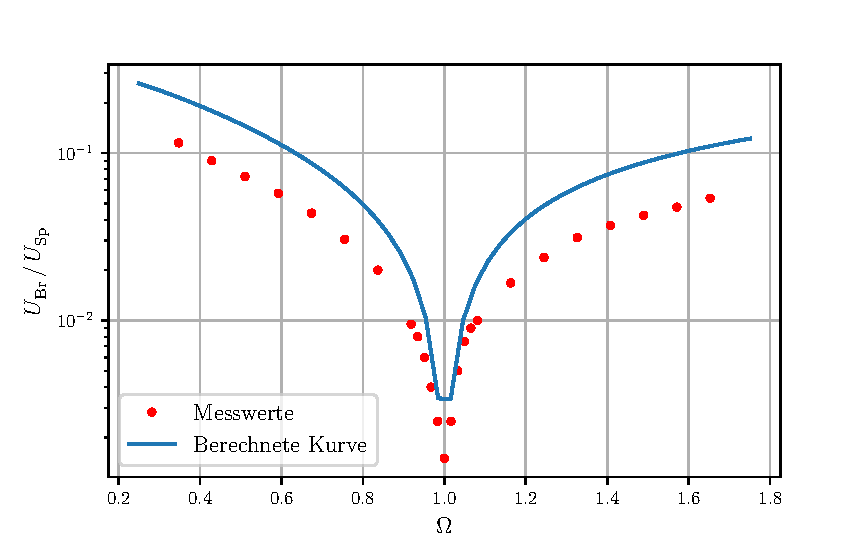
\includegraphics[width=\textwidth]{plot_wien.pdf}
    \caption{Messkurve der Wien-Robinson-Brücke.}
    \label{fig:wien}
\end{figure}

